\documentclass[conference]{IEEEtran}
\IEEEoverridecommandlockouts
% The preceding line is only needed to identify funding in the first footnote. If that is unneeded, please comment it out.
\usepackage{cite}
\usepackage{amsmath,amssymb,amsfonts}
\usepackage{algorithmic}
\usepackage{graphicx}
\usepackage{textcomp}

\usepackage[dvipsnames]{xcolor}
\usepackage{listings}

\lstdefinelanguage{Kotlin}{
  comment=[l]{//},
  commentstyle={\color{ForestGreen}\ttfamily},
  emph={value, onValueChange},
  emphstyle={\color[HTML]{467CDA}},
  identifierstyle=\color{black},
  keywords={!in, !is, abstract, actual, annotation, as, as?, break, by, catch, class, companion, const, constructor, continue, crossinline, data, delegate, do, dynamic, else, enum, expect, external, false, field, file, final, finally, for, FROM, fun, get, if, import, in, infix, init, inline, inner, interface, internal, is, lateinit, noinline, null, object, open, operator, out, override, package, param, private, property, protected, public, receiveris, reified, return, return@, sealed, SELECT, set, setparam, super, suspend, tailrec, this, throw, true, try, typealias, typeof, val, var, vararg, when, where, while},
  keywordstyle={\color[HTML]{C57531}\bfseries},
  morecomment=[s]{/*}{*/},
  morestring=[b]",
  morestring=[s]{"""*}{*"""},
  ndkeywords={@Deprecated, @Composable, @Query, @Insert, @Dao, OnConflictStrategy},
  ndkeywordstyle={\color[HTML]{BBB429}\bfseries},
  sensitive=true,
  stringstyle={\color{ForestGreen}\ttfamily},
  classoffset=2,
  morekeywords={padding, items, NavHost, composable},
  keywordstyle={\color[HTML]{FBC36B}\bfseries},
  classoffset=3,
  morekeywords={REPLACE},
  keywordstyle={\color[HTML]{9B81BC}\itshape}
}

\lstset{
    basicstyle=\ttfamily\small,
    frame=single,
    numbers=left,
    numbersep=5pt,
    numberstyle=\tiny\color{gray},
    showspaces=false,
    showstringspaces=false,
    tabsize=1,
    xleftmargin=10pt,
}

\def\BibTeX{{\rm B\kern-.05em{\sc i\kern-.025em b}\kern-.08em
    T\kern-.1667em\lower.7ex\hbox{E}\kern-.125emX}}

\begin{document}

\title{Android Jetpack}

\author{
    \IEEEauthorblockN{Tobias Fischer}
    \IEEEauthorblockA{
        University of Applied Sciences Upper Austria \\
        Faculty for Informatics, Communications and Media\\
        Degree in Mobile Computing\\
        4232 Hagenberg, Austria\\
        s2010237030@fhooe.at
    } 
    \and
    \IEEEauthorblockN{Michael Zauner}
    \IEEEauthorblockA{
        University of Applied Sciences Upper Austria \\
        Faculty for Informatics, Communications and Media\\
        Degree in Mobile Computing\\
        4232 Hagenberg, Austria\\
        s2010237032@fhooe.at
    }
}

\maketitle

\begin{abstract}
Android has a huge library landscape, although it is difficult to choose the right one. Jetpack is a collection of libraries designed to make app development easier and decrease boilerplate code. Jetpack libraries use contemporary design approaches to reduce crashes and memory leaks. This paper gives a short insight into Android Jetpack, its major libraries and its benefits and drawbacks.
\end{abstract}

\section{Introduction}
\label{cha:introduction}

Technologies are constantly changing, and this is true for Android as well. The number of libraries for Android developers is increasing rapidly, and therefore it is very difficult to choose the right ones. Furthermore, it is not an easy task to keep the architecture of an app in a manner that is easily understandable for other people. Uncontrollable growth must be prevented.

In 2018, Google has decided to give Android a new coat of paint with Android Jetpack. Android Jetpack should be a suite of libraries which should reflect the best practices in developing an Android application.

Android Jetpack is constructed like LEGO building blocks -- the libraries can be plugged together according to requirements. Splitting a framework into multiple blocks is necessary when it grows into an unmanageable state.

The most important libraries of Android Jetpack are Jetpack Compose, Room, Navigation and Databinding. According to their website \cite{android_jetpack}, Jetpack consists of almost 100 libraries (as of June 2022).

% No Sections!
% - Motivation
% - Challenges\\(Prevent impact of new features on existing concepts)
% - Goals
%    - Division into blocks for growing frameworks
%    - Module/Package (Lego)
%    - Prevent uncontrollable growth
%    - Software in continuous change (new aspects)
\section{Related Work}
\label{cha:related_work}

\subsection{General Android Libraries}
\label{cha:general_android_libs}

\noindent
\textbf{Native Libraries}

In addition to the Linux kernel layer, the Android platform contains a number of native libraries. Most of the functionality provided through the Android runtime layer is available through these native libraries \cite{cinar_2015_android_quick_apis_reference}.

According to Cinar \cite{cinar_2015_android_quick_apis_reference}, the most notable of them are:

\begin{itemize}
    \item \textit{SQLite}: in-memory, relational SQL database for persisting and accessing the application's data
    \item \textit{WebKit}: enables HTML, CSS and JavaScript to include web technology
    \item \textit{OpenGL ES}: rendering functionality (2D and 3D)
    \item \textit{Open Core}: record and play back audio and video content
    \item \textit{OpenSSL}: secure communication with SSL/TLS
\end{itemize}

\noindent
\textbf{Android Support Library}

While targeting a lower API level will increase the app's audience, it also limits the Android platform features to use. To overcome this trade-off, the Android Support Library was introduced. The Android Support Library Package is a collection of code libraries that provide backward compatible versions of recent Android APIs.
An important fact is that the Android Support Library does not cover every new API because sometimes new OS features are required \cite{cinar_2015_android_quick_apis_reference}.
\section{Android Jetpack}
\label{cha:android_jetpack}

\subsection{Jetpack in general}
\label{cha:jetpack_general}

Jetpack is a set of many useful libraries which are used in Android development. It combines old and new libraries, therefore managing and updating gets much easier. As of 2018 when Jetpack got announced at the Google I/O one of the first steps was to rename the old \textit{android.support.*} libraries which are used for compatibility across multiple Android versions, to the new namespace \textit{androidx.*} \cite{allen2021introducingandroid}.

The components used in Jetpack are not bundled and each one must be imported explicitly. The available parts can be categorized into four categories, as shown in figure~\ref{fig:jetpack_components}. The categories are architecture, user interface, foundation and behavior. Which components are in which category is shown in the following figure:

\begin{figure}[ht]
  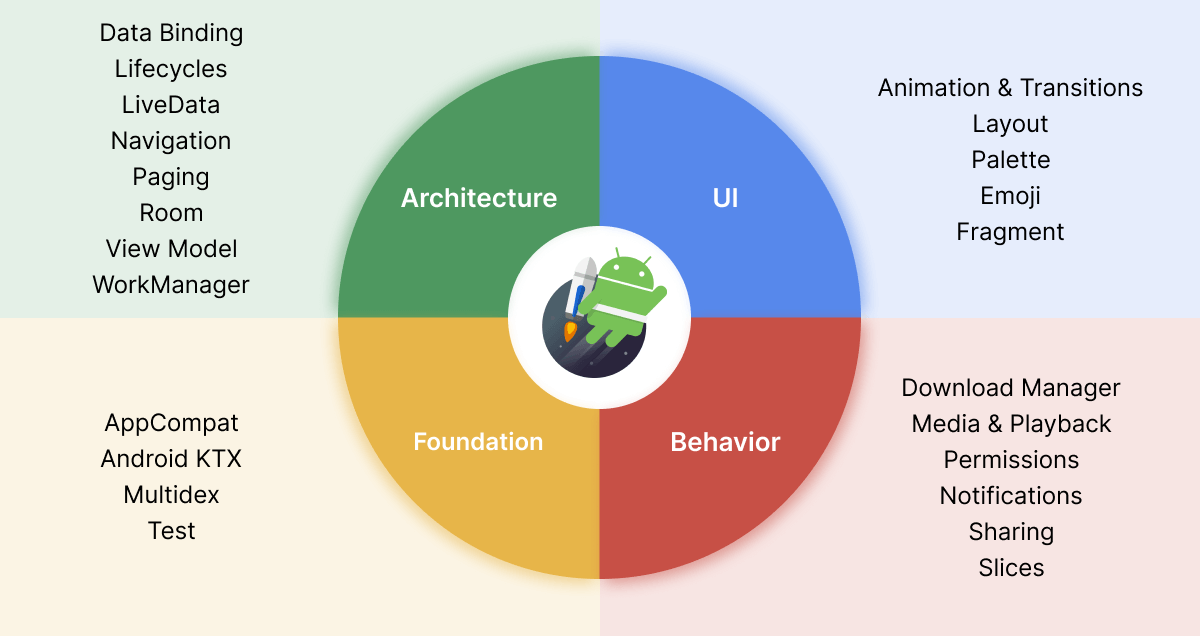
\includegraphics[width=\linewidth]{images/android-jetpack-components.png}
  \caption{Jetpack components and its categories \cite{Figure_1}}
  \label{fig:jetpack_components}
\end{figure}
% https://img.orangesoft.co/media/android-jetpack-components.png

One of the major goals of Jetpack is the integration with the programming language \textit{Kotlin}.
At the Google I/O 2019, Google announced the future development of Android will be written in Kotlin, because you can code more cleaner code than with the boilerplate language \textit{Java}. Kotlin and Java are 100\% interoperable, which means you can call Kotlin-code from Java and call Java-code from Kotlin \cite{android_kotlin_first}.
    
% \cite{android_jetpack_google}
\subsection{Jetpack Compose}
\label{cha:compose}

The biggest renewal of the Android framework comes with Jetpack Compose. Compose is a new UI framework for Android. According to the statements of Google \cite{android_jetpack_compose} the framework speeds up UI development, requires less code, and has many powerful tools.

Compared to building the UI implicitly in XML files, Jetpack Compose is meant to be declarative. Declarative UI allows to put design and programmatic logic in one single file  \cite{android_jetpack_compose}. Some other popular examples using this approach are React, Flutter, SwiftUI and many more.

\noindent
The main benefits according to the "Android for Developers" web page \cite{android_jetpack_compose} are:
\begin{itemize}
    \item less Code
    \item intuitive
    \begin{itemize}
        \item writing code in Kotlin (declarative)
        \item Android takes care of the rest
    \end{itemize}
    \item accelerate Development
    \item powerful
    \item performs better than XML
    \item usage alongside existing code
    \item test integration
\end{itemize}

Besides the list of advantages, there are also some drawbacks of using Jetpack Compose:

\begin{itemize}
    \item a lot of magic happens in the background
    \item difficult to understand
    \item the preview is in a early state and leads to some teething troubles \\
\end{itemize}

\noindent
\textbf{Declarative Programming Paradigm}

In the old approach (imperative), the layout is built with a tree of UI widgets. There, the state changes of the application need to be updated manually with methods like \lstinline[language=Kotlin]{setText(String)} or \lstinline[language=Kotlin]{setVisibility(Integer)}. This technique is very error prone because a update of those widgets could be missing at some point. Another error cause is that the view was removed from the UI and creates an illegal state \cite{android_thinking_in_compose}.

To avoid these errors, the declarative approach has been developed in recent years. This approach describes the desired end result and what it should look like, instead of listing all the execution steps that would lead to a result. On every state change the entire screen gets regenerated from scratch which could be very expensive in terms of time, computing power and battery usage. Therefore Compose tries in the Recomposition process to choose the parts which have to be redrawn and the other ones are skipped. Recomposition is performed only on objects that are intended to change. \cite{android_thinking_in_compose}. \\

\noindent
\textbf{Composable Functions}

The basic functionality of Compose is relying on composable functions. Composable functions convert data into UI elements, so they may have parameters and they do not return anything. Instead of returning something, the functions are describing the screen state instead of building UI widgets. These functions are annotated with \lstinline[language=Kotlin]{@Composable} annotation. Another important fact is that it is not possible to set or get the function. It simply can be overwritten by calling the same functions with other arguments \cite{android_thinking_in_compose}.

A simple composable function that displays "Hello" with a name specified in the parameter:

\begin{lstlisting}[language=Kotlin]
@Composable
fun Greeting(name: String) {
    Text("Hello $name!")
}
\end{lstlisting}

In the matter of fact that composable functions are written in Kotlin, it is possible to use loops (for, while, \ldots), contitions (if, when, \ldots) or any other logical construct \cite{android_thinking_in_compose}. \\

\noindent
Some other important facts from the Google documentation \cite{android_thinking_in_compose} are as follows:
\begin{itemize}
    \item Composable functions can execute in any order and parallel
    \item Recomposition ignores composable functions and lambdas where possible
    \item Recomposition is optimistic (restarts recomposition again whenever a new parameter arrives)
    \item Composable functions should be very fast as they might run quite frequently (can lead to poor performance if this is not followed) \\
\end{itemize}

\noindent
\textbf{Managing States}

The only way to update the UI is by calling the same composable with new arguments \cite{android_state_compose}. For state changes, functionality is needed that saves a state and calls the current composable again with new arguments to redraw the UI. This basic functionality is implemented as follows:

\noindent
\lstinline[language=Kotlin]|var state by remember {mutableStateOf("")}| \\

A composable function can store a single object in memory by usage by of \lstinline[language=Kotlin]|remember| keyword. During composition the value is stored and the value gets returned while recomposition. Therefore, the value can be used with the variable (for example \lstinline[language=Kotlin]{state}) during the recomposition process.

The delegated property \lstinline[language=Kotlin]|mutablestateof| creates a observable which would schedule a recomposition of any composable function which reads the changed value. \cite{android_state_compose}

An example of saving the state of a text field and using the "Greeting" function shown earlier:

\begin{lstlisting}[language=Kotlin]
@Composable
fun SomeInputText() {
    var name by remember { 
        mutableStateOf("World") 
    }
    
    Greeting(name)
    TextField(
        value = name,
        onValueChange = { name = it }
    )
}
\end{lstlisting}

\noindent
\textbf{Phases}

Jetpack Compose renders each frame in three different phases. In the standard Android View system, the three phases are called Measure -- Layout -- Drawing. Instead of the Measure phases, Compose has a phase called Composition.

The phases mentioned in the Android Developer platform \cite{android_compose_phases} are as follows:

\begin{itemize}
    \item Composition: Which parts of the user interface should be displayed?
    \item Layout: Where to place objects on the UI?
    \item Drawing: How to render the UI?  \\
\end{itemize}

\noindent
\textbf{Architectural Layering}

Since Jetpack Compose consists of more than one project, it is assembled from several modules to form a complete stack.

\noindent
The major layers are \cite{android_compose_layering}:
\begin{itemize}
    \item Material: implementation of Material Design (theming system, designed components, ripple displays, icons, \ldots)
    \item Foundation: system independent building blocks (\lstinline[language=Kotlin]|Row|, \lstinline[language=Kotlin]|Column|, \lstinline[language=Kotlin]|LazyColumn|, \ldots)
    \item UI: basic UI capabilities (\lstinline[language=Kotlin]|Modifier|, \ldots)
    \item Runtime: provides fundamental functionality (\lstinline[language=Kotlin]|remember|, \lstinline[language=Kotlin]|mutableStateOf|, \lstinline[language=Kotlin]|@Composable|, \ldots) 
\end{itemize}

\noindent
\textbf{Example of the "new" RecyclerView}

RecyclerView were used to represent a list of data on the UI. Every old RecyclerView needs an Adapter with a ViewHolder and produces much boiler plate code. Compose introduces the \lstinline[language=Kotlin]|LazyColumn| and \lstinline[language=Kotlin]|LazyRow| and therefore no longer requires RecyclerViews.

An example of creating a list with LazyColumn:

\begin{lstlisting}[language=Kotlin]
LazyColumn(Modifier.padding(it)){
    items(someList) { someItem ->
        Text(someItem)
    }
}
\end{lstlisting}
\subsection{Room}
\label{cha:room}

In comparison of using Shared Preferences instead of Room it is possible to persist non-trivial amounts of structured data. The Room persistence library provides an abstraction layer over the SQLite database. It allows easier access to the database, but uses SQLite in the background.
The most important benefits are \cite{android_room}:

\begin{itemize}
    \item compile-time validation of SQL queries
    \item minimizes boilerplate code with annotations
    \item enables migrations \\
\end{itemize}

\noindent
The major components of Android Room are \cite{android_room}:

\begin{itemize}
    \item Database Class: main access point for the database connection
    \item Data Entities: tables of database
    \item Data Access Objects (DAOs): methods for querying, updating and deleting data in the database \\
\end{itemize}

In \cite{Figure_2} it is shown how theses components work together. The Room Database get the queries from the DAO and executes them. The result will then be stored in the entities via the getter/setter methods.

\begin{figure}[ht]
    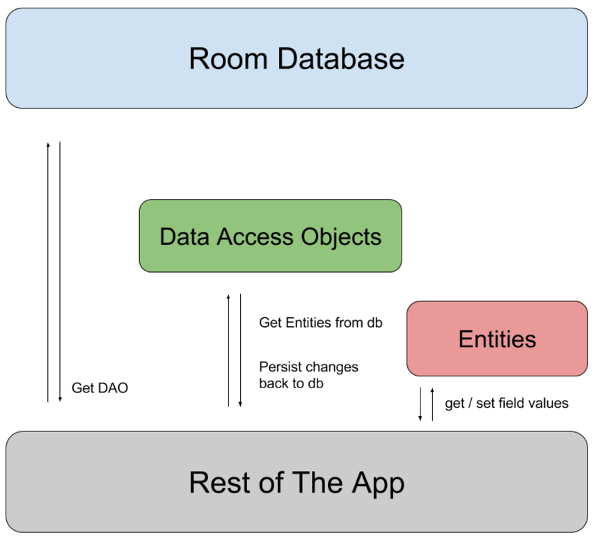
\includegraphics[width=\linewidth]{images/room_architecture.png}
    \caption{Architecture of Room \cite{Figure_2}}
    \label{fig:room_architecture}
\end{figure}

Example of a DAO for some table supporting a select, insert and delete statement:

\begin{lstlisting}[language=Kotlin]
@Dao
interface SomeTableDao {
    /**
     * @return all entries
     */
    @Query("SELECT * FROM some_table")
    fun getAll(): Flow<List<SomeEntry>>

    /**
     * insert a range of entries
     */
    @Insert(onConflict = 
        OnConflictStrategy.REPLACE
    )
    fun insertAll(vararg entries: SomeEntry)

    /**
     * delete all entries
     */
    @Query("DELETE FROM some_entry")
    fun deleteAll()
}
\end{lstlisting}
\subsection{Navigation}
\label{cha:navigation}

The interactions that let users move between, inside, and outside of the various pieces of content in a app are referred to as navigation. The Navigation component of Android Jetpack assists in implementing navigation, from straightforward button clicks to more intricate patterns like app bars and the navigation drawer. The navigation component also ensures a consistent and predictable user experience by adhering to a set of principles \cite{android_navigation}.

The main navigation concept conists of three major parts:
\begin{itemize}
    \item NavController manages the navigation workflow. When a new destination should be visible, the NavController sends the UI elements to the NavHost. It also take care of the Back Stack when interacting with different destinations. When the user wants to go back, the NavController know exactly which destination was the previous one. The controller is read out as follows:
    
    \noindent
    \lstinline{val navController = rememberNavController()}
    
    \item NavHost is a container which displays the composable functions of the destinations. Here follows an example:
    
\begin{lstlisting}[language=Kotlin]
val start = "screen1"
NavHost(navController, start) {
    composable("screen1") {
        Screen1()
    }
    composable("screen2") {
        Screen2()
    }
}
\end{lstlisting}

    \item Navigation Graph: defines the possible ways to navigate through the application. Before Jetpack Compose this component was declared in a XML file, where the single destinations and the interactions between them can be defined. Like in this example \cite{Figure_3} you define a start destination and from there on you have 2 different possible ways to navigate through the application. You can go to the registration or view the leader board.
    
    \begin{figure}[ht]
        \centering
        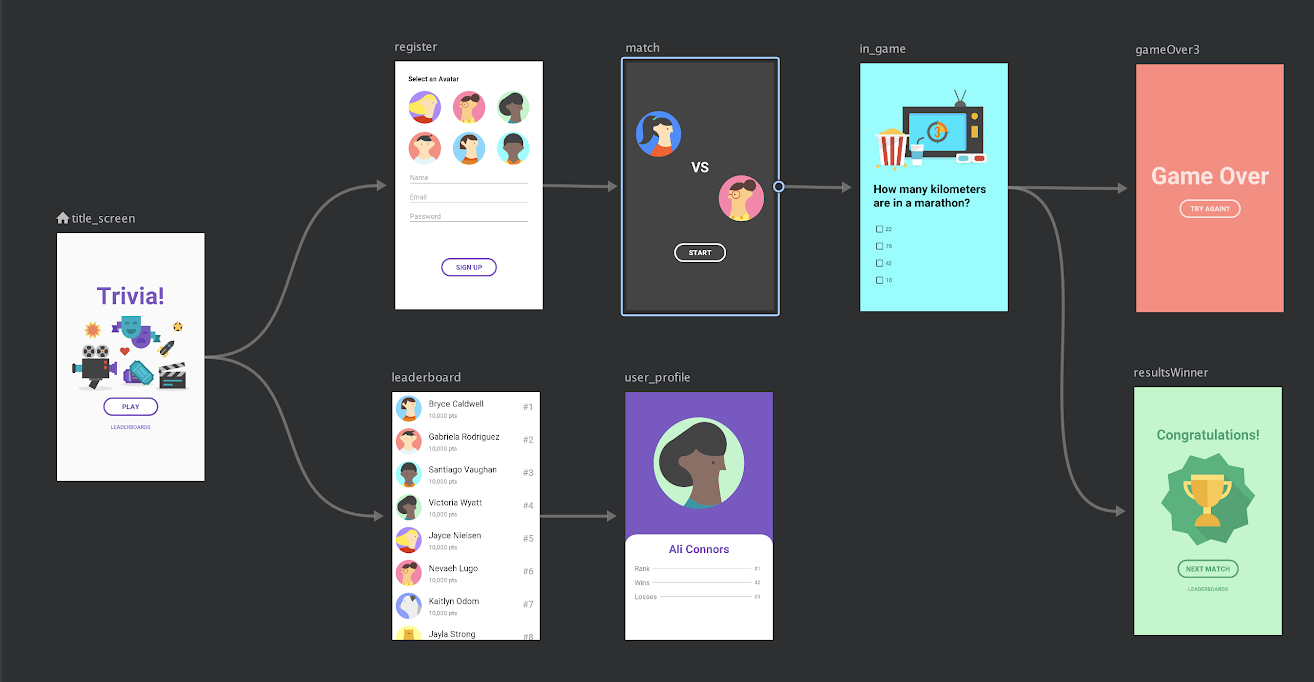
\includegraphics[width=\linewidth]{images/navigation_graph.png}
        \caption{Example navigation graph \cite{Figure_3}}
        \label{fig:navgraph}
    \end{figure}
    % https://miro.medium.com/max/1400/1*ESf1y0VYcHE5ldkCDD8HKA.png
    
\end{itemize}
\subsection{Interacting with ViewModels and Kotlin Flows}
\label{cha:jetpack_interacting}

\noindent
\textbf{Asynchronous Data}

Flow is a datatype introduced in Kotlin Coroutines and it is used to collect data which changes in the background (e.g.: updating news from a website). Normally non-simultaneous functions return a single value, but what if you need multiple values? This is where Flow comes into action. It generates a continuous data stream where you can attach to it and collect its asynchronous data. A Flow consists of two parts\cite{android_flows}:
\begin{itemize}
    \item \textit{producer}: provides the data stream (mostly asynchronous due to Coroutines) using \textit{emit()}
    \item \textit{consumer}: fetches the data and do other processing (e.g: displaying in UI) using \textit{collect()} \\
\end{itemize}

\noindent
\textbf{ViewModel}

A ViewModel is designed to store and handle UI relevant data in an application, taking into account the Android lifecycle. It holds the states and values of its objects (e.g.: like a Flow list of news) regardless of system configuration changes (e.g.: changing screen orientation). ViewModel is a observable holder for data and you can get notified when the data changes. In a modern application architecture a ViewModel transforms the data from a repository (local or remote source) to a Flow/LiveData list. When ever the list content changes it will update the UI.

A \lstinline[language=Kotlin]|@Composable| function can collect the asynchronous data from a ViewModel as a state. Whenever a change in the data is recognized, the value of the variable will be changed and it will automatically update the UI (if the data needs to be displayed)
\section{Conclusion}
\label{cha:conclusion}

The Android development world is growing rapidly. It is hard for developers to stay up-to-date all the time. Libraries and APIs are constantly changing. Google tries to counter this problem with Android Jetpack. They provide a collection of libraries to help developers cope with this problem. With Jetpack, developers have all the tools to create a modern android application.

On the other hand, Jetpack also has a not-so-good side. For example, it is hard for people who learned Android programming the older way, like the XML-style UI, to switch to the declarative UI of Jetpack Compose. Everything they learned about fragments is different now, because fragments just don't exist anymore. There are only Composable functions left to interact with the UI.

Jetpack has a great documentation about all components and also the GitHub account of Google is a great starting point. They provide coding examples to get in touch with the best coding practices in Android development. It just takes some time to get used to a new style of programming. But it is definitely recommended for an Android beginner to start with the old XML-style UI because it necessary to learn about the components a application really has and how these work together. Jetpack Compose does a lot of magic in the background and when someone really wants to learn Android development it is necessary to know what these magically short code snippets really do. Currently another big drawback is, that some features of Jetpack are not yet mature enough (for example the preview of Jetpack Compose).

To sum it up, Android Jetpack is really great. Room, Navigation and Android KTX (Kotlin extensions) make most of the developers happy, it simplifies so many things and saves the lifes from bad practices. Jetpack Compose will be the future of UI development, but it will take some time to adapt to this new style. Everybody is looking forward for the new handy libraries in Android Jetpack.

\graphicspath{{images/}}

\bibliographystyle{IEEEtran}
\bibliography{references} % Biblatex-Literaturdatei (references.bib)

\end{document}